\documentclass[12pt,a4paper]{article}

\usepackage[T1]{fontenc}
\usepackage[utf8]{inputenc}
\usepackage[brazil]{babel}
\usepackage{lmodern}
\usepackage{geometry}
\usepackage{hyperref}
\usepackage{enumitem}
\usepackage{array}
\usepackage{amsmath}
\usepackage{graphicx}
\usepackage{xcolor}
\usepackage{booktabs}
\usepackage{listings}

\graphicspath{{./}{../../01-Aulas/assets/}{../../01-Aulas/img/apostila/}}

\geometry{margin=2.5cm}
\hypersetup{
  colorlinks=true,
  linkcolor=blue,
  urlcolor=blue
}

\definecolor{codebg}{RGB}{245, 246, 248}
\definecolor{codeborder}{RGB}{220, 224, 230}
\definecolor{codekw}{RGB}{0, 92, 197}
\definecolor{codecm}{RGB}{80, 95, 110}

\lstdefinestyle{sql}{
  basicstyle=\ttfamily\small,
  backgroundcolor=\color{codebg},
  frame=single,
  rulecolor=\color{codeborder},
  breaklines=true,
  columns=fullflexible,
  keepspaces=true,
  showstringspaces=false,
  keywordstyle=\color{codekw}\bfseries,
  commentstyle=\color{codecm}\itshape,
  tabsize=2,
  language=SQL
}

\lstdefinestyle{text}{
  basicstyle=\ttfamily\small,
  backgroundcolor=\color{codebg},
  frame=single,
  rulecolor=\color{codeborder},
  breaklines=true,
  columns=fullflexible,
  keepspaces=true,
  showstringspaces=false,
  tabsize=2
}

\title{Apostila Completa --- Banco de Dados 1}
\date{}

\begin{document}
\maketitle

\noindent
\textbf{Público-alvo:} Iniciantes\\
\textbf{Objetivo:} Sair do conceito (ER) até implementação, consultas, qualidade, automações e transações.\\
\textbf{Como usar:} Leia os exemplos, copie os modelos e resolva os exercícios ao final de cada capítulo.

\tableofcontents
\newpage

\section{Fundamentos: dado, informação, BD e SGBD}

\subsection{Dado vs.\ informação}
\textbf{Dado} é um fato bruto (ex.: ``Maria'', ``25'', ``Belo Horizonte''). \textbf{Informação} é dado com contexto (ex.: ``Maria tem 25 anos e mora em Belo Horizonte'').
\begin{center}
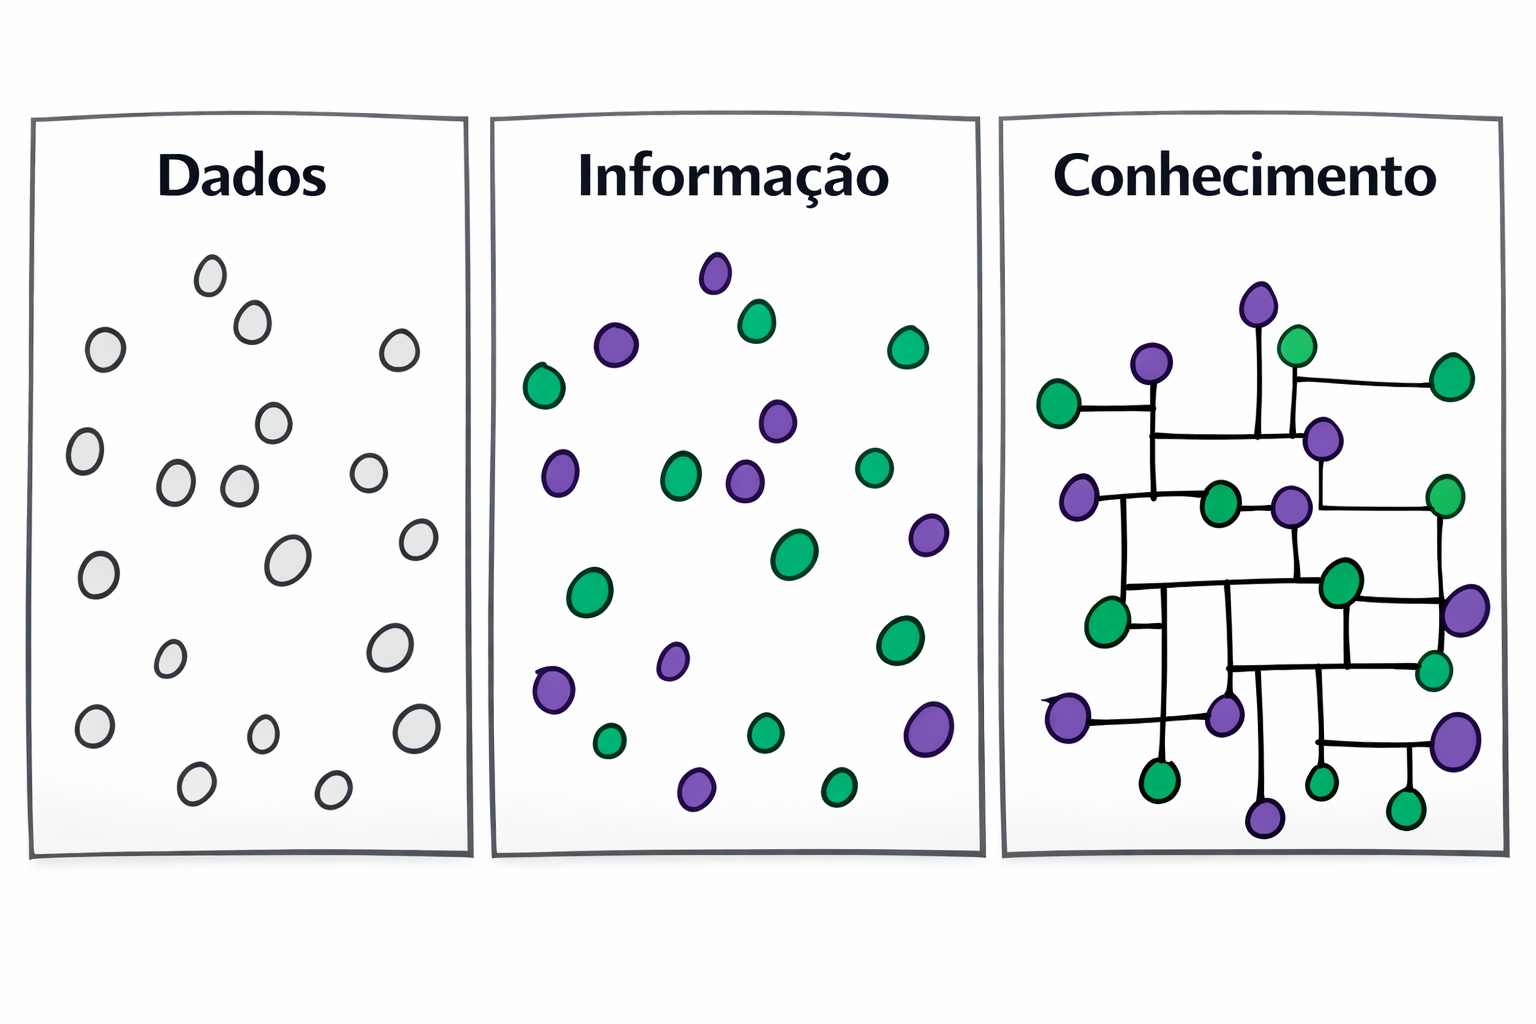
\includegraphics[width=0.95\textwidth]{dadoxinfo.png}
\end{center}
\noindent
\textbf{Explicação da imagem:}
\begin{itemize}[leftmargin=*,itemsep=0.2em]
  \item \textbf{Dados:} pontos soltos. São valores isolados (fatos brutos) sem significado por si só.
  \item \textbf{Informação:} dados organizados (por categoria/ordem/contexto). Ao agrupar e descrever, você passa a entender o que eles representam.
  \item \textbf{Conhecimento:} conexões entre informações. As relações/padrões permitem explicar, prever e tomar decisões.
\end{itemize}

\subsection{Banco de Dados e SGBD}
\textbf{Banco de Dados (BD)} é o conjunto organizado de dados. \textbf{SGBD} é o software que gerencia o BD (armazenar, consultar, controlar acesso e consistência), por exemplo: PostgreSQL, MySQL, SQL Server, Oracle.
\begin{center}
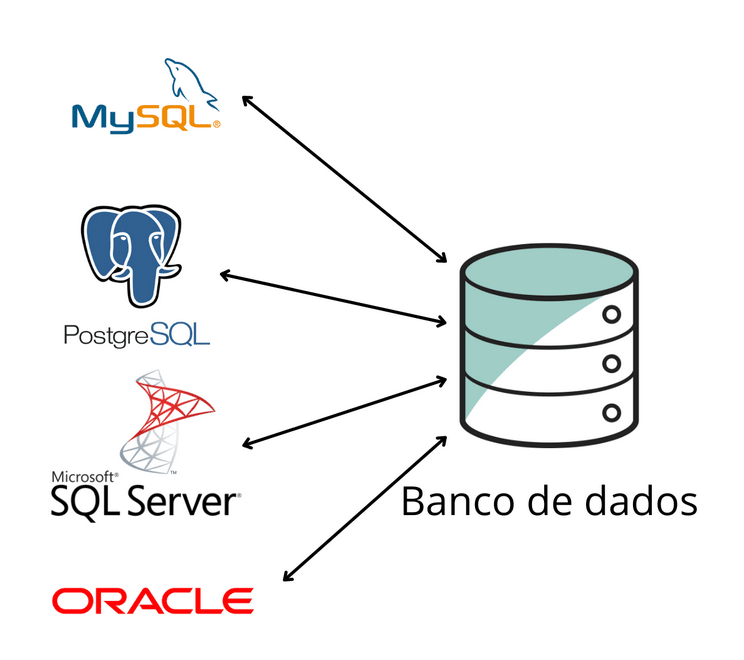
\includegraphics[width=0.9\textwidth]{sgbd.png}
\end{center}

\subsection{Modelo relacional: a linguagem do armazenamento}
\begin{itemize}[leftmargin=*,itemsep=0.2em]
  \item \textbf{Tabela (relação):} conjunto de registros do mesmo tipo.
  \item \textbf{Coluna (atributo):} característica de cada registro.
  \item \textbf{Linha (tupla/registro):} um item completo.
  \item \textbf{Chave Primária (PK):} identifica unicamente uma linha.
  \item \textbf{Chave Estrangeira (FK):} referencia uma PK em outra tabela.
\end{itemize}

\subsection{Modelo pronto: ficha de requisitos do domínio}
\begin{lstlisting}[style=text]
Domínio:

Entidades principais (coisas sobre as quais guardamos dados):

Regras de negócio (frases do mundo real):
1)
2)
3)

Operações que o sistema precisa responder (perguntas):
1)
2)
3)
\end{lstlisting}

\section{Modelagem Conceitual: Entidade-Relacionamento (ER)}

\subsection{Elementos do ER}
\begin{itemize}[leftmargin=*,itemsep=0.2em]
  \item \textbf{Entidade:} coisa sobre a qual registramos dados (Cliente, Produto, Pedido).
  \item \textbf{Atributo:} característica (Nome, CPF, Preço).
  \item \textbf{Relacionamento:} ligação (Cliente faz Pedido).
  \item \textbf{Cardinalidade:} 1:1, 1:N, N:M.
\end{itemize}

\subsection{Relacionamento 1:1 (um para um)}
\begin{center}
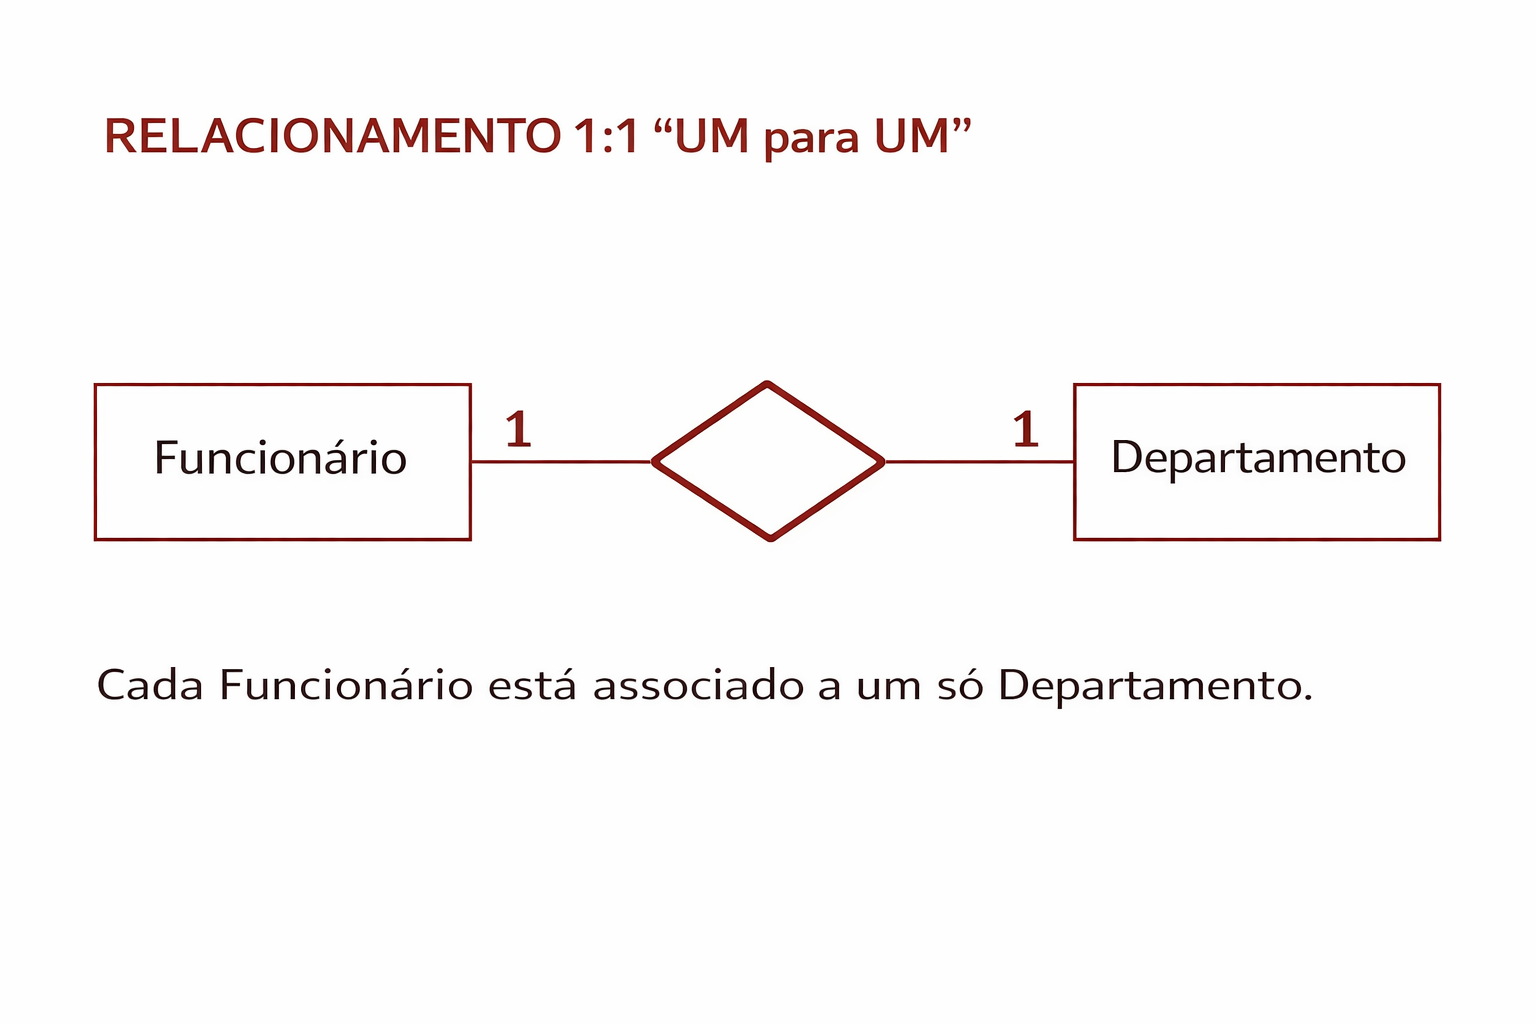
\includegraphics[width=0.95\textwidth]{ralaciona1.png}
\end{center}
\noindent
\textbf{Como interpretar 1:1:}
\begin{itemize}[leftmargin=*,itemsep=0.2em]
  \item Cada instância de uma entidade se relaciona com \textbf{no máximo uma} instância da outra.
  \item No exemplo, cada \textbf{Funcionário} está associado a um só \textbf{Departamento} e cada \textbf{Departamento} se associa a um só \textbf{Funcionário}.
  \item Atenção: o ``1'' indica quantidade máxima; a \textbf{participação} pode ser obrigatória (deve) ou opcional (pode), dependendo da regra do domínio.
\end{itemize}

\subsection{Checklist rápido de qualidade do ER}
\begin{itemize}[leftmargin=*,itemsep=0.2em]
  \item Nomes de entidades no singular e claros.
  \item Atributos atômicos (sem listas dentro do atributo).
  \item Cada entidade com identificador (candidato a PK).
  \item Cardinalidades justificadas por uma frase do domínio.
  \item N:M identificado e tratado (normalmente vira tabela associativa no relacional).
\end{itemize}

\subsection{Exemplo completo: Biblioteca (modelo conceitual)}
\textbf{Regras do domínio (exemplo):}
\begin{itemize}[leftmargin=*,itemsep=0.2em]
  \item Um \textbf{Usuário} pode realizar vários \textbf{Empréstimos}.
  \item Um \textbf{Empréstimo} refere-se a um \textbf{Livro}.
  \item Um \textbf{Livro} pode ter um ou mais \textbf{Autores}.
\end{itemize}

\textbf{Sugestão de entidades e atributos:}
\begin{itemize}[leftmargin=*,itemsep=0.2em]
  \item USUARIO(\underline{id\_usuario}, nome, email, telefone)
  \item LIVRO(\underline{id\_livro}, titulo, isbn, ano)
  \item AUTOR(\underline{id\_autor}, nome)
  \item EMPRESTIMO(\underline{id\_emprestimo}, data\_emprestimo, data\_prevista, data\_devolucao)
\end{itemize}

\textbf{Visual (referência):} se desejar, use a imagem abaixo como exemplo de diagrama.

\begin{center}
\includegraphics[width=0.95\textwidth]{A01biblioteca_er.png}
\end{center}

\subsection{Modelo pronto: roteiro para extrair ER de um texto}
\begin{lstlisting}[style=text]
1) Sublinhe substantivos: possíveis entidades.
2) Circule verbos/frases de ação: possíveis relacionamentos.
3) Liste atributos para cada entidade.
4) Defina identificadores (candidatos a PK).
5) Para cada relacionamento, escreva a frase: "Quantos X para um Y?"
6) Desenhe e revise com checklist de qualidade.
\end{lstlisting}

\section{Do ER para tabelas: Mapeamento ER $\rightarrow$ Relacional}

\subsection{Regras essenciais (prático)}
\begin{itemize}[leftmargin=*,itemsep=0.2em]
  \item \textbf{Entidade $\rightarrow$ tabela:} atributos simples viram colunas; identificador vira PK.
  \item \textbf{Relacionamento 1:N:} FK do lado 1 vai para o lado N.
  \item \textbf{Relacionamento 1:1:} FK em um dos lados (geralmente no lado opcional) ou mesclar.
  \item \textbf{Relacionamento N:M:} criar tabela associativa com duas FKs; PK pode ser composta.
  \item \textbf{Atributos do relacionamento:} vão para a tabela do relacionamento (em N:M, na associativa).
\end{itemize}

\subsection{Exemplo: Matrícula (N:M com atributos)}
\textbf{Domínio:} Aluno se matricula em Disciplina. A matrícula tem data e status.

\begin{itemize}[leftmargin=*,itemsep=0.2em]
  \item ALUNO(\underline{id\_aluno}, nome, email)
  \item DISCIPLINA(\underline{id\_disciplina}, nome, carga\_horaria)
  \item MATRICULA(\underline{id\_aluno}, \underline{id\_disciplina}, data\_matricula, status)
\end{itemize}

\subsection{Modelo pronto: dicionário de dados}
\begin{lstlisting}[style=text]
Tabela:
Descrição:

Coluna | Tipo | Nulo? | Regras | Exemplo
------ | ---- | ----- | ------ | -------
id     |      |       | PK     |
\end{lstlisting}

\section{Álgebra Relacional (pensar antes da sintaxe)}

\subsection{Ideia central}
Consultas podem ser vistas como \textbf{operações} sobre conjuntos de tuplas.

\subsection{Operações mais usadas}
\begin{itemize}[leftmargin=*,itemsep=0.2em]
  \item \textbf{Seleção ($\sigma$):} filtra linhas por condição.
  \item \textbf{Projeção ($\pi$):} seleciona colunas.
  \item \textbf{Junção (join):} combina informações entre tabelas relacionadas.
  \item \textbf{União e diferença:} operações entre relações compatíveis.
\end{itemize}

\subsection{Exemplo (conceitual) com clínica}
\textbf{Seleção:} $\sigma_{\text{cidade = ``BH''}}(\text{CLIENTE})$\\
\textbf{Projeção:} $\pi_{\text{nome}}(\text{CLIENTE})$\\
\textbf{Junção:} $\text{CLIENTE} \bowtie_{\text{CLIENTE.id = PET.id\_cliente}} \text{PET}$

\section{SQL: DDL e DML (criar e manipular dados)}

\subsection{Esquema exemplo: Clínica Veterinária}
\begin{lstlisting}[style=sql]
CREATE TABLE cliente (
  id_cliente INTEGER PRIMARY KEY,
  nome       VARCHAR(120) NOT NULL,
  telefone   VARCHAR(30),
  cidade     VARCHAR(80)
);

CREATE TABLE pet (
  id_pet     INTEGER PRIMARY KEY,
  id_cliente INTEGER NOT NULL,
  nome       VARCHAR(120) NOT NULL,
  tipo       VARCHAR(40) NOT NULL,
  CONSTRAINT fk_pet_cliente
    FOREIGN KEY (id_cliente)
    REFERENCES cliente (id_cliente)
);
\end{lstlisting}

\subsection{Inserções e alterações (com boas práticas)}
\begin{lstlisting}[style=sql]
INSERT INTO cliente (id_cliente, nome, telefone, cidade)
VALUES
  (1, 'Maria Silva', '31999990000', 'Belo Horizonte'),
  (2, 'Joao Souza',  '31988880000', 'Contagem');

INSERT INTO pet (id_pet, id_cliente, nome, tipo)
VALUES
  (10, 1, 'Luna', 'Gato'),
  (11, 1, 'Thor', 'Cachorro'),
  (12, 2, 'Nina', 'Cachorro');

UPDATE cliente
SET telefone = '31977770000'
WHERE id_cliente = 1;

DELETE FROM pet
WHERE id_pet = 12;
\end{lstlisting}

\subsection{Modelo pronto: script base de banco}
\begin{lstlisting}[style=sql]
BEGIN;

DROP TABLE IF EXISTS tabela_filha;
DROP TABLE IF EXISTS tabela_pai;

CREATE TABLE tabela_pai (
  id INTEGER PRIMARY KEY
);

CREATE TABLE tabela_filha (
  id INTEGER PRIMARY KEY,
  id_pai INTEGER NOT NULL,
  FOREIGN KEY (id_pai) REFERENCES tabela_pai (id)
);

COMMIT;
\end{lstlisting}

\section{SQL: Consultas, agregações e JOINs}

\subsection{Consultas básicas}
\begin{lstlisting}[style=sql]
SELECT id_cliente, nome, cidade
FROM cliente
WHERE cidade = 'Belo Horizonte'
ORDER BY nome;

SELECT id_pet, nome, tipo
FROM pet
WHERE tipo = 'Cachorro'
ORDER BY nome;
\end{lstlisting}

\subsection{JOIN: trazendo o nome do cliente para cada pet}
\begin{lstlisting}[style=sql]
SELECT
  p.id_pet,
  p.nome   AS nome_pet,
  p.tipo,
  c.nome   AS nome_cliente,
  c.cidade
FROM pet p
JOIN cliente c
  ON c.id_cliente = p.id_cliente
ORDER BY c.nome, p.nome;
\end{lstlisting}

\subsection{Agregações e HAVING}
\begin{lstlisting}[style=sql]
SELECT
  c.id_cliente,
  c.nome,
  COUNT(*) AS qtd_pets
FROM cliente c
JOIN pet p
  ON p.id_cliente = c.id_cliente
GROUP BY c.id_cliente, c.nome
HAVING COUNT(*) >= 2
ORDER BY qtd_pets DESC, c.nome;
\end{lstlisting}

\subsection{Modelo pronto: tradução de pergunta para SQL}
\begin{lstlisting}[style=text]
Pergunta:

Tabelas envolvidas:

Filtros (WHERE):

Junções (JOIN ... ON):

Agrupamento (GROUP BY):

Regras após agrupar (HAVING):

Ordenação (ORDER BY):
\end{lstlisting}

\section{Qualidade do esquema: dependência funcional e normalização}

\subsection{Problema: redundância e anomalias}
Quando a mesma informação é repetida em várias linhas, surgem inconsistências. Exemplo: telefone do cliente repetido em cada pedido. Se mudar, você precisa atualizar tudo.

\subsection{Dependência funcional}
Uma dependência funcional $X \rightarrow Y$ significa que $X$ determina $Y$. Em geral, uma \textbf{chave} determina todos os demais atributos da tabela.

\subsection{Formas normais (até 3FN, na prática)}
\begin{itemize}[leftmargin=*,itemsep=0.2em]
  \item \textbf{1FN:} sem grupos repetidos; atributos atômicos.
  \item \textbf{2FN:} sem dependência parcial em chave composta.
  \item \textbf{3FN:} sem dependência transitiva (atributo não-chave determinando outro).
\end{itemize}

\subsection{Exemplo guiado: tabela bagunçada}
\begin{center}
\begin{tabular}{@{}lllll@{}}
\toprule
id\_pedido & nome\_cliente & telefone & id\_produto & nome\_produto \\
\midrule
101 & Maria Silva & 31999990000 & 5 & Racao X \\
102 & Maria Silva & 31999990000 & 7 & Coleira Y \\
\bottomrule
\end{tabular}
\end{center}

\textbf{Decomposição sugerida:}
\begin{itemize}[leftmargin=*,itemsep=0.2em]
  \item CLIENTE(\underline{id\_cliente}, nome, telefone)
  \item PRODUTO(\underline{id\_produto}, nome)
  \item PEDIDO(\underline{id\_pedido}, id\_cliente)
  \item ITEM\_PEDIDO(\underline{id\_pedido}, \underline{id\_produto})
\end{itemize}

\section{Procedimentos armazenados (procedures)}

\subsection{Quando usar}
\begin{itemize}[leftmargin=*,itemsep=0.2em]
  \item Reutilizar lógica de negócio comum.
  \item Validar entradas antes de inserir/atualizar.
  \item Centralizar regras e reduzir repetição no aplicativo.
\end{itemize}

\subsection{Modelo pronto (pseudocódigo adaptável ao SGBD)}
\begin{lstlisting}[style=sql]
-- Ajuste a sintaxe para o seu SGBD (PostgreSQL, MySQL, etc.)
-- Objetivo: cadastrar pet apenas se cliente existir.
\end{lstlisting}

\subsection{Exemplo (PostgreSQL): função para cadastrar pet}
\begin{lstlisting}[style=sql]
CREATE OR REPLACE FUNCTION cadastrar_pet(
  p_id_pet INTEGER,
  p_id_cliente INTEGER,
  p_nome VARCHAR,
  p_tipo VARCHAR
)
RETURNS VOID
LANGUAGE plpgsql
AS $$
BEGIN
  IF NOT EXISTS (SELECT 1 FROM cliente WHERE id_cliente = p_id_cliente) THEN
    RAISE EXCEPTION 'Cliente % nao existe', p_id_cliente;
  END IF;

  INSERT INTO pet (id_pet, id_cliente, nome, tipo)
  VALUES (p_id_pet, p_id_cliente, p_nome, p_tipo);
END;
$$;
\end{lstlisting}

\section{Asserções, constraints e gatilhos (triggers)}

\subsection{Constraints primeiro}
Antes de criar triggers, tente resolver com constraints: PK, FK, UNIQUE, CHECK e NOT NULL.

\subsection{Trigger: auditoria simples}
\begin{lstlisting}[style=sql]
CREATE TABLE log_pet (
  id_log     INTEGER GENERATED ALWAYS AS IDENTITY PRIMARY KEY,
  id_pet     INTEGER NOT NULL,
  operacao   VARCHAR(10) NOT NULL,
  momento    TIMESTAMP NOT NULL DEFAULT CURRENT_TIMESTAMP
);
\end{lstlisting}

\subsection{Exemplo (PostgreSQL): trigger para logar DELETE}
\begin{lstlisting}[style=sql]
CREATE OR REPLACE FUNCTION log_pet_delete()
RETURNS TRIGGER
LANGUAGE plpgsql
AS $$
BEGIN
  INSERT INTO log_pet (id_pet, operacao)
  VALUES (OLD.id_pet, 'DELETE');
  RETURN OLD;
END;
$$;

CREATE TRIGGER trg_pet_delete
AFTER DELETE ON pet
FOR EACH ROW
EXECUTE FUNCTION log_pet_delete();
\end{lstlisting}

\section{Transações e ACID}

\subsection{Ideia: tudo ou nada}
Uma transferência bancária tem dois passos (debitar e creditar). Se um falhar, o estado não pode ficar pela metade.

\subsection{Modelo pronto: transação de transferência}
\begin{lstlisting}[style=sql]
BEGIN;

UPDATE conta
SET saldo = saldo - 100
WHERE id_conta = 1;

UPDATE conta
SET saldo = saldo + 100
WHERE id_conta = 2;

COMMIT;
\end{lstlisting}

\subsection{Exemplo: rollback forçado}
\begin{lstlisting}[style=sql]
BEGIN;

UPDATE conta
SET saldo = saldo - 100
WHERE id_conta = 1;

-- Simule um erro aqui (ou uma regra de negocio falha)
ROLLBACK;
\end{lstlisting}

\section{Exercícios (com gabarito curto)}

\subsection{Exercício 1: ER a partir de texto (Biblioteca)}
\textbf{Enunciado:} Uma biblioteca possui usuários e livros. Um usuário realiza empréstimos de livros. Um livro pode ter vários autores e um autor pode ter vários livros. Um empréstimo tem data de empréstimo e data de devolução.

\textbf{Tarefa:} proponha entidades, atributos, identificadores e cardinalidades.

\textbf{Gabarito (exemplo):}
\begin{itemize}[leftmargin=*,itemsep=0.2em]
  \item USUARIO(\underline{id\_usuario}, nome, email)
  \item LIVRO(\underline{id\_livro}, titulo, isbn)
  \item AUTOR(\underline{id\_autor}, nome)
  \item EMPRESTIMO(\underline{id\_emprestimo}, id\_usuario, id\_livro, data\_emprestimo, data\_devolucao)
  \item LIVRO\_AUTOR(\underline{id\_livro}, \underline{id\_autor})
\end{itemize}

\subsection{Exercício 2: SQL (consultas)}
\textbf{Enunciado:} usando o esquema CLIENTE e PET:
\begin{itemize}[leftmargin=*,itemsep=0.2em]
  \item Liste todos os pets de um cliente pelo nome do cliente.
  \item Conte quantos pets cada cliente possui.
\end{itemize}

\textbf{Gabarito (exemplo):}
\begin{lstlisting}[style=sql]
SELECT p.*
FROM pet p
JOIN cliente c
  ON c.id_cliente = p.id_cliente
WHERE c.nome = 'Maria Silva'
ORDER BY p.nome;

SELECT c.nome, COUNT(*) AS qtd_pets
FROM cliente c
JOIN pet p
  ON p.id_cliente = c.id_cliente
GROUP BY c.nome
ORDER BY qtd_pets DESC, c.nome;
\end{lstlisting}

\subsection{Exercício 3: normalização}
\textbf{Enunciado:} proponha uma decomposição para uma tabela que mistura aluno, disciplina e professor, onde um professor tem sala fixa.

\textbf{Gabarito (exemplo):}
\begin{itemize}[leftmargin=*,itemsep=0.2em]
  \item PROFESSOR(\underline{id\_professor}, nome, sala)
  \item ALUNO(\underline{id\_aluno}, nome)
  \item DISCIPLINA(\underline{id\_disciplina}, nome)
  \item TURMA(\underline{id\_turma}, id\_disciplina, id\_professor)
  \item MATRICULA(\underline{id\_aluno}, \underline{id\_turma})
\end{itemize}

\end{document}
